\chapter{Machine Learning}
\label{chapter:MachineLearning}

\section{Introduction}

As described in Section~\ref{sec:MultiLabelBinaryClassification}, to reconstruct tracks from the reconstructed hits in an event, one must solve a multi-label binary classification problem. This chapter describes how Machine Learning addresses this question.

\ \\Since the labels are known, the task is a supervised problem. Supervised learning can be either classification or regression. Since the labels have categorical values of +1 or -1, this is a classification problem. There are several types of classification problems.

\ \\Multi-class is a classification with more than two classes. In this category each sample is assigned to one and only one label. For example, a colour can have only one label from several choices: red, green, or blue. In other words, there is only one question, and the answer to each question can be one of three or more labels.

\ \\Multi-label is a classification where each sample is mapped to a set of labels, each being binary. This is like asking several questions, the answer to each being either yes or no. In this case, the question asked is if the output is +1 or -1 for the hit. Therefore, this is a multi-label classsificaton problem.

\ \\The general case is a multi-class multi-label classification problem: where there are many questions, the answer to each being selected from a finite set of categorical labels. 

\section{Neural Network Architecture}

Several machine learning algorithms can be used to perform a classification task. The most common are decision trees and neural networks~\cite{AndrewNg}. Several decision trees are trained and grouped together into an ensemble method such as random forests and boosted decision trees. In general, to find a multi-dimensional function representing a non-linear relation between input and output, it is efficient to train a neural network (NN). NNs are statistical models inspired by biological neural networks in the brain. The brain contains millions of neuron cells forming a network where electro-chemical impulses are passed between them. An artificial neural network is formed by a number of interconnected artificial \emph{neurons}, or \emph{nodes}. In this project NNs are used.

\ \\One NN characteristic is that they contain weights along paths between neurons. The weights can be tuned with an algorithm that learns from observed data to improve the model. The NN learns through optimisation techniques, like gradient descent. A NN is represented by an architecture formed by layers of artificial neurons, which are able to receive several inputs. Each input is processed by an activation function to determine the output. A simple model is formed by an input layer followed by a single hidden layer and then an output layer. Each layer may contain one or more neurons. A NN with more than one hidden layer is called a deep neural network (DNN). For the best DNN performance, the model has to be designed according to the problem being solved, and then the hyper-parameters are tuned. A general structure of a fully connected DNN is presented in Figure~\ref{fig:DNN}.

\begin{figure}[h]
  \centering
  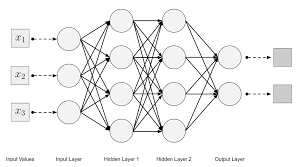
\includegraphics[width=0.6\textwidth]{./plots/DNNArchitecture.png}
  \caption{Diagram of the general architecture of a DNN. Credit image: O'Reilly.~\cite{OReilly}.}
  \label{fig:DNN}
\end{figure}

\ \\The \emph{Universal Approximation Theorem} states that a neural network with one \emph{hidden layer} can in principle approximate any N-dimensional function to an arbitrary degree of accuracy, given a sufficiently large (though finite) number of nodes. In practice however, it is more suitable to use multiple hidden layers connected in series~\cite{AndrewNg}.

\ \\In a fully connected NN, each node takes a weighted linear combination of the outputs from nodes of the previous layer, adds its own bias value, and applies an \emph{activation function}. The node output represents the input to neurons of the next layer, as illustrated in Figure~\ref{fig:Neuron}. The activation function is chosen via optimisation for each neuron when the architecture of the NN is defined. 

\begin{figure}[h]
  \centering
  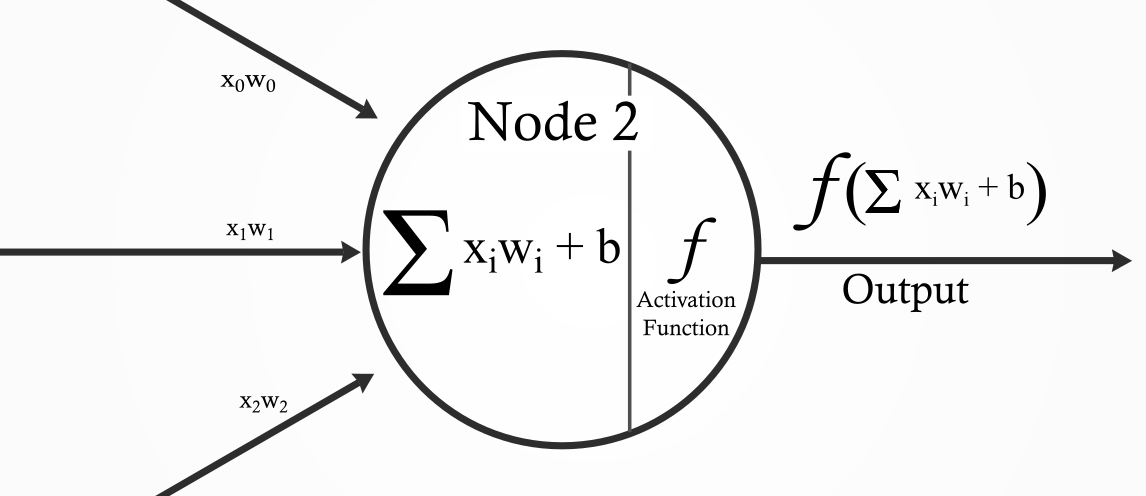
\includegraphics[width=0.6\textwidth]{./plots/Neuron.png}
  \caption{Diagram of a neuron or node in a NN, with its weight inputs, bias and the output via the activation function. Credit image: The Fork~\cite{TheFork}.}
  \label{fig:Neuron}
\end{figure}

\ \\Once the NN architecture (the layers, nodes and activation functions) is defined, the total function of the NN is parametrised by all the weights for connections between nodes plus the biases of each node. Training the NN means learning these weights and biases so that the NN can predict the output when new data not seen before is taken as input.

\section{Hyper-Parameters}
\label{sec:Hyperparameters}

Several hyper-parameter choices can be made depending on the question being asked: the number of hidden layers, number of nodes on a hidden layer, the activation function of nodes in the hidden layers, the activation function of nodes in the output layer, the learning optimizer, the loss function, and the batch size. In the plots of this section the hyper-parameters that are retained for the best performing model are coloured in red, to illustrate their performance relative to other possible hyper-parameters.

\ \\The problem is a multi-label binary classification. Given a collection (bucket) of 20 hits, the question is whether the hit belongs to the particle with the largest number of hits in the bucket. If the hit belongs to the majority particle, the label +1 is applied, otherwise the label 0 or -1 is applied. A preliminary study suggests that the latter option using a label of -1 provides better results. With this choice, there remains only a limited number of appropriate activation functions for the output layer and loss functions. 

\ \\Firstly, the output value of the NN prediction fixes the choice of the activation function on the last layer to the hyperbolic tangent (TANH), which has values between -1.0 and 1.0. The logistic regression function, also called sigmoid, is not appropriate because it has values between 0.0 and 1.0, illustrated in Equations

\begin{equation}
   \tanh x = \frac{\sinh x}{\cosh x} = \frac{e^x - e^{-x}}{e^x + e^{-x}} = \frac{e^{2x}-1}{e^{2x}+1}
\end{equation}

\ \\and

\begin{equation}
   S(x) = \frac{1}{1 + e^{-x}} = \frac{e^{x}}{e^{x}+1}.
\end{equation}

\ \\and on the left-hand side of Figure~\ref{fig:ActivationFunctionsLastLayer}. Two more activation functions are possible for values between -1.0 and 1.0. The square non linear (SQNL) is described by Equation

\begin{equation}
   \SQNL~(x) = 
\begin{dcases}
    -1 , & x < -2.0\\
    x + \frac{x^2}{4}, & -2.0 \leq x < 0\\
    x - \frac{x^2}{4}, & 0 \leq x < 2.0\\   
    1 , & x > 2.0\\
\end{dcases}.
\end{equation}

\ \\ and the soft sign (SOSI) function by Equation

\begin{equation}
   \SOSI~(x) = \frac{x}{1 + |x|}.
\end{equation}

\ \\All three functions reach the values of -1.0 and 1.0, though for different values of x. SQNL, TANH and SOSI reach the value of 1.0 (-1.0) for x values of exactly 2.0 (-2.0), of around $\pi \sim 3.14$ (-$\pi \sim -3.14$) and for $\infty$ ($-\infty$), respectively, as illustrated in the right-hand side of Figure~\ref{fig:ActivationFunctionsLastLayer}.

\begin{figure}[htb]
\centering
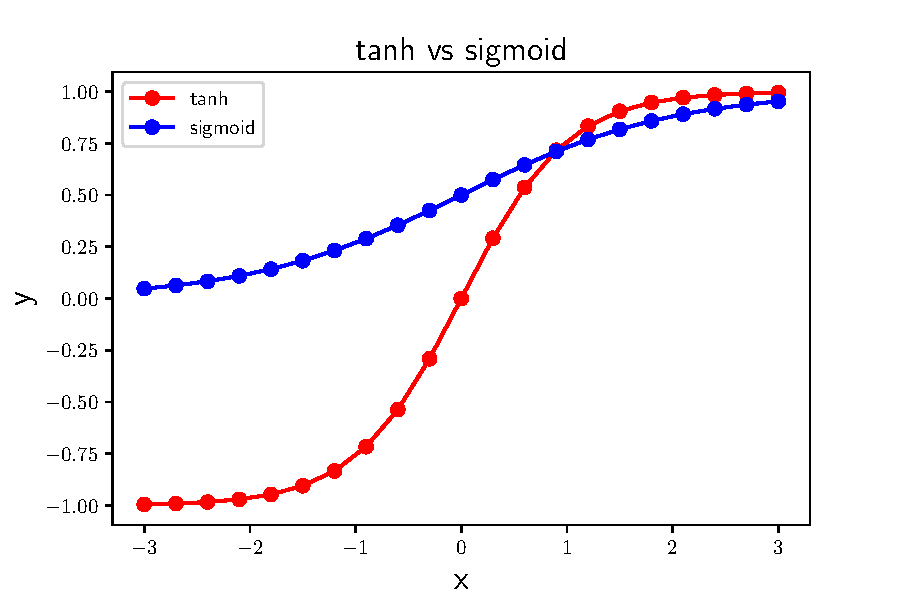
\includegraphics[width=0.45\textwidth]{plots/ActivationFunctionsLastLayer1.pdf}
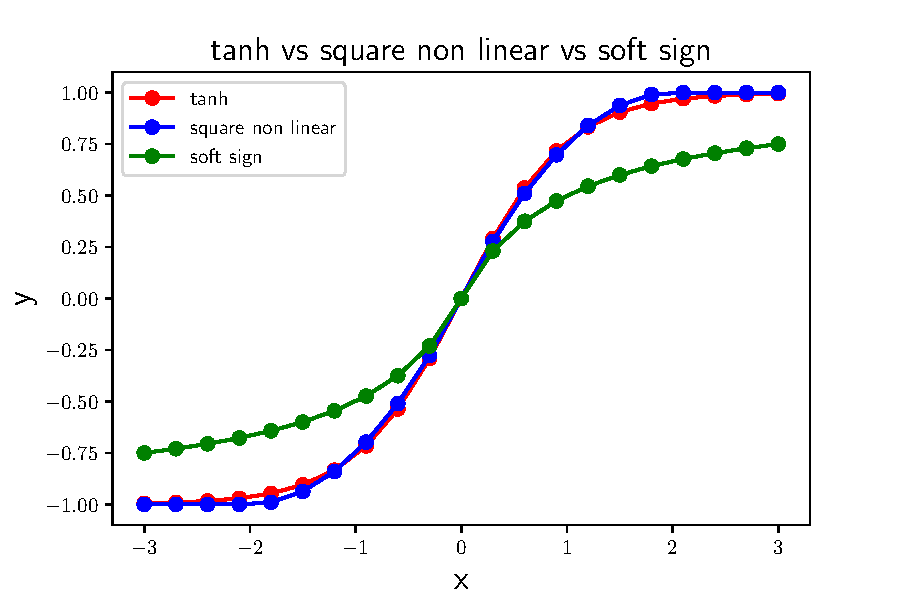
\includegraphics[width=0.45\textwidth]{plots/ActivationFunctionsLastLayer2.pdf}
\caption{Overlaid potential activation functions for the final layer. Left: hyperbolic tangent (tanh) and logistic regression (sigmoid). Right: tanh, square non linear and soft sign. tanh is chosen as our output labels are -1.0 and 1.0.}
\label{fig:ActivationFunctionsLastLayer}
\end{figure}

\ \\There are only two appropriate loss functions for the target values of -1.0 and 1.0: the (regular) hinge function and the squared hinge function. Denoting $y$ the predicted output and $t$ the true target output (label), the hinge function is given by Equation

\begin{equation}
   \LossFunctionHinge:~l(y) = \max(0, 1 - t \cdot y),
\end{equation}

\ \\and the squared hinge by Equation

\begin{equation}
   \LossFunctionSquaredHinge:~l(y) = [\max(0, 1 - t \cdot y)]^2.
\end{equation}

\ \\Their relative behaviour is illustrated in Figure~\ref{fig:LossFunctions} for $t=-1.0$ (left) and $t=1.0$ (right). These loss functions never become negative. For $t=1.0$, for $y \ge t$, the loss function is exactly zero. For $y<t$, the loss function gradually increases. The squared hinge does not have a discontinuity at $y=1.0$ and at high values increases more than the regular hinge, applying a bigger penalty for large deviations. The same is valid for $y=-1.0$, but in the opposite direction. 

\begin{figure}[htb]
\centering
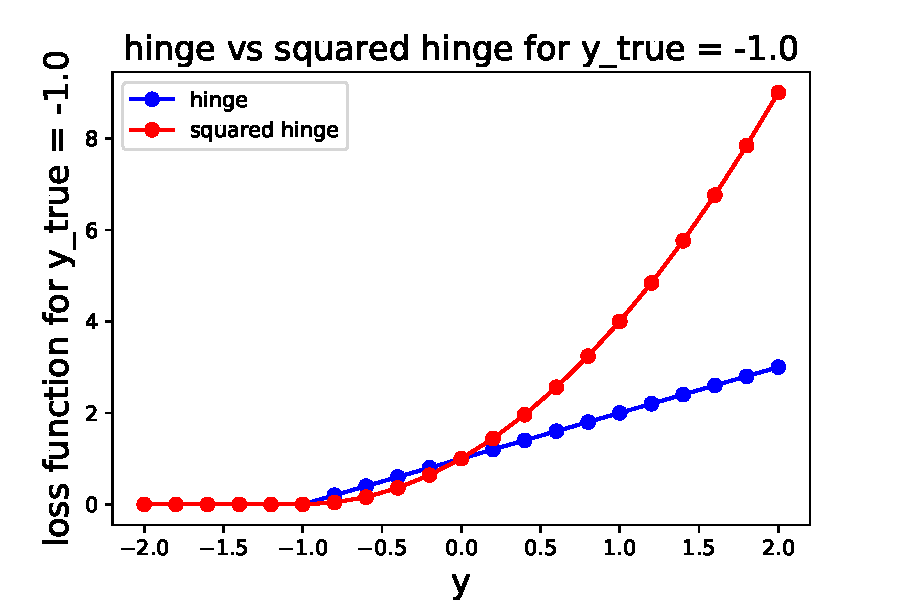
\includegraphics[width=0.45\textwidth]{plots/LossFunctions_MinusOne.pdf}
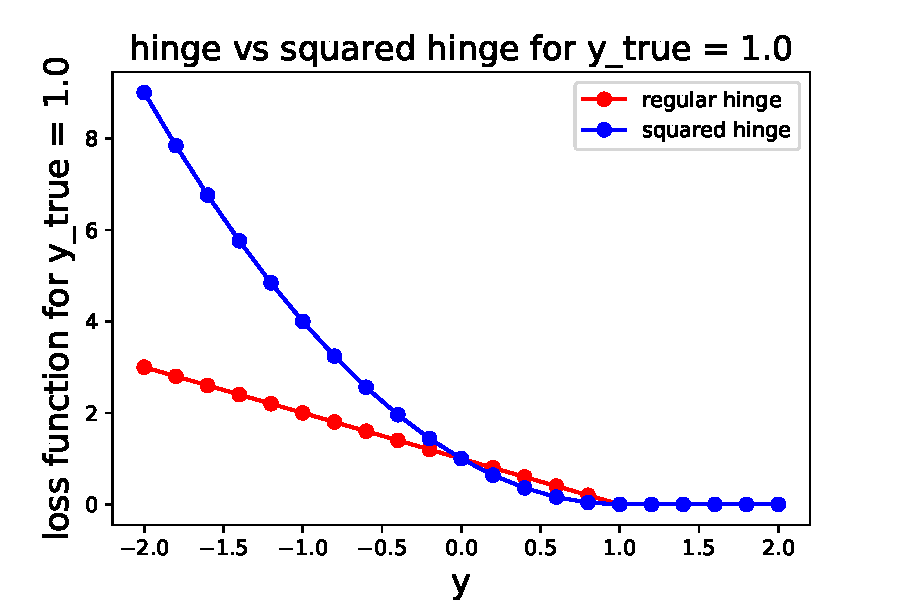
\includegraphics[width=0.45\textwidth]{plots/LossFunctions_PlusOne.pdf}
\caption{Overlaid loss functions of (regular) hinge and squared hinge for varying predicted $y$, for a fixed true $y$ of -1.0 (left) and 1.0 (right).}
\label{fig:LossFunctions}
\end{figure}

\ \\The functions above apply to a pair of predicted $y$ and true $t$ values. In this problem, a loss function must be evaluated for each hit. The final loss function for the entire sample represents a sum over all the buckets in all events, and for each bucket the sum over each of the 20 hits, as exemplified in Equations

\begin{equation}
   \LossFunctionHinge:~l(y) = \sum_{\rm bucket} \sum_{\rm hit} \max(0, 1 - t_{\rm hit} \cdot y_{\rm hit})
\end{equation}

\ \\ and

\begin{equation}
   \LossFunctionSquaredHinge:~l(y) = \sum_{\rm bucket} \sum_{\rm hit} [\max(0, 1 - t_{\rm hit} \cdot y_{\rm hit})]^2.
\end{equation}

\ \\Another choice to make is that of the activation functions for the nodes of the hidden layers. Besides the already-mentioned sigmoid and hyperbolic tangent functions, the Rectified Linear Unit (ReLU) is introduced. ReLU is a common activation function for neural networks, including for more advanced neural networks such as convolutional neural networks (CNN) or deep neural networks (DNN). ReLU is \emph{rectified} from the bottom, meaning its values are zero for negative inputs and return the same value as the input for positive inputs. ReLU can be summarized by Equation

\begin{equation}
   \ReLU:~R(x)= \max(0, x).
\end{equation}

\ \\While both the function R(x) and its derivative are monotonic, the function also has some drawbacks. Firsly, it is not differentiable at zero. Secondly, since for all negative values the input is exactly zero, for methods learning with gradient descent, the ability to learn is reduced. To address this problem, a variation of ReLU is introduced, namely the Exponential Linear Function (ELU), described by Equation

\begin{equation}
     \ELU:~E(x= 
\begin{dcases}
    \alpha(e^x -1), & x < 0\\
    x,              & x \geq 0
\end{dcases}.
\end{equation}

\ \\For positive values, the function remains the same. But for negative values, an exponential curve appears, tending smoothly to a constant value $\alpha$. ELU has several advantages over ReLU: it is fully continuous and differentiable, and does not have the vanishing gradient problem for gradient descent learning. Its main disadvantage is that it is slower to compute for negative values, but this may be worth it for a more precise result. The comparison of the ReLU and ELU functions is illustrated in Figure~\ref{fig:ActivationFunctionsHiddenLayers}.

\begin{figure}[htb]
\centering
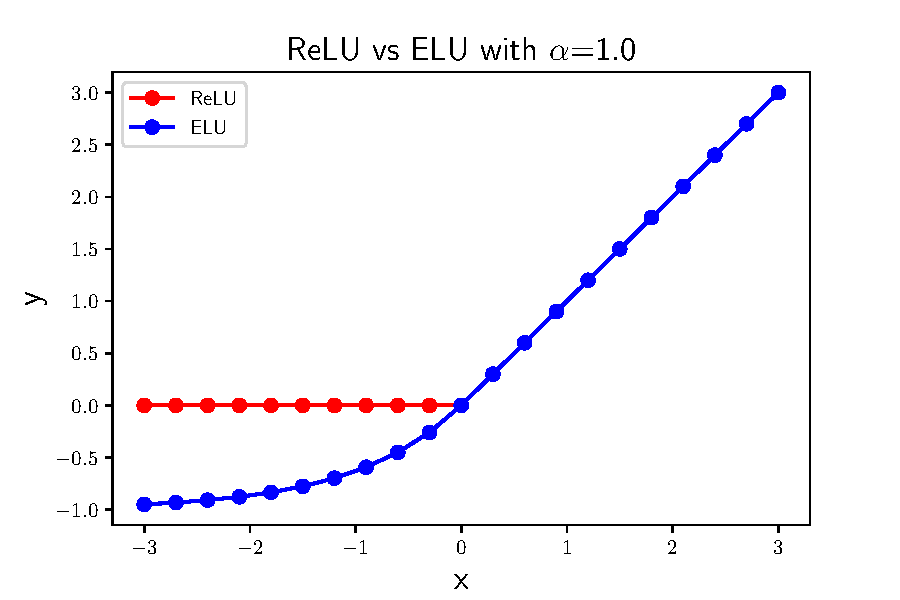
\includegraphics[width=0.45\textwidth]{plots/ActivationFunctionsHiddenLayers.pdf}
\caption{Overlaid activation functions of ReLU and ELU, with $\alpha=1.0$}
\label{fig:ActivationFunctionsHiddenLayers}
\end{figure}

\ \\Another hyper-parameter to tune is the number of hidden layers and the number of nodes on each hidden layer. The \emph{Universal Approximation Theorem} suggests that one layer with a very large number of nodes is enough to learn any arbitrary function. But in practice it is worth having several consecutive layers of fewer nodes per layer. That forms a deep neural network. 

\ \\Another option in the architecture of the NN is whether to use a regularisation layer, in particular a dropout layer~\cite{DropoutLayer}. Sometimes the resulting model is too complex relative to the quantity of input data, leading to overfitting during training. Overfitting is similar to memorisation of the input data, leading to not be able to predict correctly on new data. To avoid overfitting, regularisation techniques are used. Typical methods add a new term to the loss functions. Other techniques add a dropout layer. The dropout method randomly sets some of the inputs to 0.0 with a frequency $f$, and reweights the other inputs by $1/(1-f)$, so that the total sum of inputs remains constant. The value of $f$ is a hyper-parameter to be optimised. The location of the dropout layer is usually between the hidden layers and the final layer. The dropout method is applied only during training, and not during testing or infering on new data.

\ \\Another choice related to the learning method is the learning optimiser. Two algorithms based on stochastic gradient descent are compared, namely Adam~\cite{Adam} and AdaDelta~\cite{AdaDelta}. For both, their default parameters are used, the most important being the learning rate of 0.001. Adam is very computationally efficient, while AdaDelta uses an adaptive learning rate. 

\section{Learning Methods}

NN training learns on the training dataset and tests on the testing dataset, described in Section~\ref{sec:TrainAndTest}. Running once over all the data from training and testing represents an \emph{epoch}. During an epoch, events are analysed in groups called \emph{batches}. The number of epochs to run and the number of events in each batch can be optimised.

\ \\Let's take a look at how the NN training happens. At first, the NN has random values for the weights and biases. For each of the events in the first batch, data comes in, and the NN predicts output values. At first these are very different from the true desired output value. To evaluate how far away the predicted output is from the desired output, a \emph{loss} function is defined that can be chosen from several formulas, but have the generic form of a sum over the absolute values of the difference. The goal of the NN training is to update the values of the weights and biases so that the loss function is minimized. After the first batch, the NN changes the weights via a back-propagation algorithm using the optimiser algorithm. For each new batch, the weights and biases change, and become continously closer to the correct values, as the loss function becomes gradually smaller. When all the training events are used, the first epoch is finished. The NN function at this point is then applied to the testing dataset, which is not split in batches, and a loss function is also calculated. The entire procedure repeats for the number of epochs chosen. At the end, the final weights and biases define the final NN model that has been learned.

\section{Train and Test Split and k-fold}
\label{sec:TrainAndTest}

The k-fold validation is a procedure used to test the effectiveness of a machine learning model. It is used especially if the data are limited. Normally, the data are split in two equal parts (train and test), corresponding to k=2. For a general k, the data are split randomly into k groups. k-1 groups are used in training and the last one is used in testing. The operation is repeated by permuting the groups, so that each group is used only once in testing. The final result is obtained by averaging out the permutations.

\ \\The split between train and test does not have to be done in equal parts. In this project the split is done with k=2, 70\% in train and 30\% in test. There are 100 events. Since by the laws of particle physics, events simulate independent particle collisions, one strategy is to divide the events randomly. As NN training takes a significant amount of time, it is useful to be able to check whether the performance has reached a plateau. In each step of 10 events, the first 7 are used for training (Train sample) and the following 3 events are used for testing (Test sample). After each step, a check is made whether the performance has reached a plateau. The pseudo-code is described in Appendix~\ref{sec:AppendixPseudoCodeInputOutput}.

\section{Balancing Datasets}
\label{sec:BalancingDatasets}

It is common practice in ML classification problems that the signal is much rarer than the background. This is called an unbalanced dataset. The solution is to balance the dataset by increasing the weights of signal events such that the total sum of weights of signal equals the total sum of weights for background. NN learning uses these weights. A balanced dataset is used for training, without a bias towards one category or the other. For testing, the unbalanced dataset is used in order to represent the real-world situation where the balancing ratio is not known.

\ \\From studies in Chapter~\ref{chapter:TrackML}, it is decided that all buckets with fewer than 10 hits with label +1, have their label set to -1. This has the result that buckets with \nbPositiveHit~between 1 and 9 now have \nbPositiveHit~of 0. 

\ \\The NN training performs better if equal number of buckets are given for each value of \nbPositiveHit. For this reason, a number of buckets with \nbPositiveHit~between 10 and 16 are removed such that there remain equal number of buckets with \nbPositiveHit~between 10 and 17. No buckets are removed with \nbPositiveHit~between 18 and 20, as they are already too few.

\ \\The two operations above make the dataset even more unbalanced towards the negative hits. For the final rebalancing of positive and negative hits, a number of buckets with \nbPositiveHit=0 are removed, such the total number of positive and negative hits in the sample are equal. About 130k buckets remain in the balanced training dataset. The testing set remains unbalanced, with roughly 3.2M buckets.

\section{Hyper-Parameter Tuning}
\label{sec:HyperparameterTuning}

The hyper-parameters are tuned by choosing the models that perform best in the test sample over 300 epochs. The performance metrics used are the accuracy and loss that result directly from Keras/TensorFlow after the training. In the plots of this section, the best model summarised in Section~\ref{sec:BestModel} is compared with alternative models where all hyper-parameters are kept constant, except one that is changed. Training on 1200 epochs on an unbalanced test dataset takes too long. For this reason, for the purpose of choosing the best hyper-parameters the test dataset is also balanced, and only 300 epochs are used. The performance of the best model is evaluated when trained in 1200 epochs on the unbalanced test dataset, as described in Chapter~\ref{chapter:ModelPerformance}. From this study the best performining hyper-parameters are chosen. When the performance of several hyper-parameters is similar, the simplest or most commonly used hyper-parameter is chosen. The resulting final model is presented in Section~\ref{sec:BestModel}.

\subsection{DNN Architecture}
\label{sec:DNNArchitecture}

A comparison of the number of hidden layers is studied. The performance is similar for different values, and 3 hidden layers is retained for the final model, as it provides a slightly better performance, as illustrated in Figure~\ref{fig:HPNbHiddenLayers}.

\begin{figure}[htb]
\centering
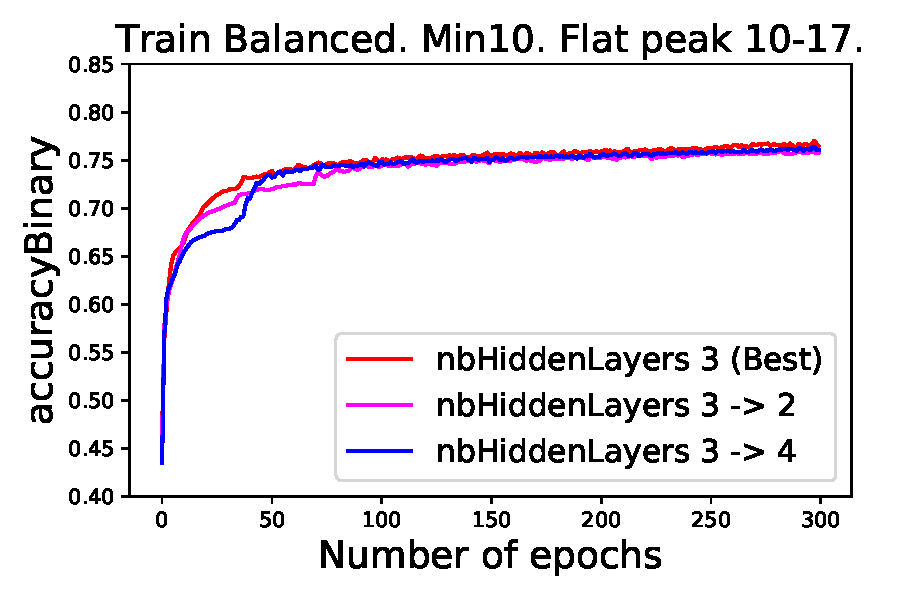
\includegraphics[width=0.32\textwidth]{plots/plot_01_1_overlay_graph_accuracyBinary_Train_NbHiddenLayers.pdf}
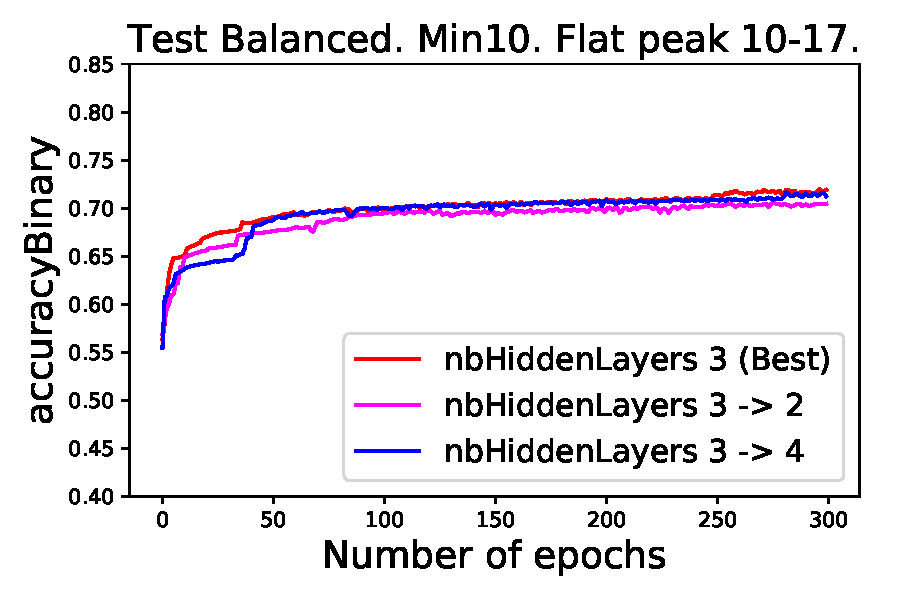
\includegraphics[width=0.32\textwidth]{plots/plot_01_1_overlay_graph_accuracyBinary_Test_NbHiddenLayers.pdf}\\
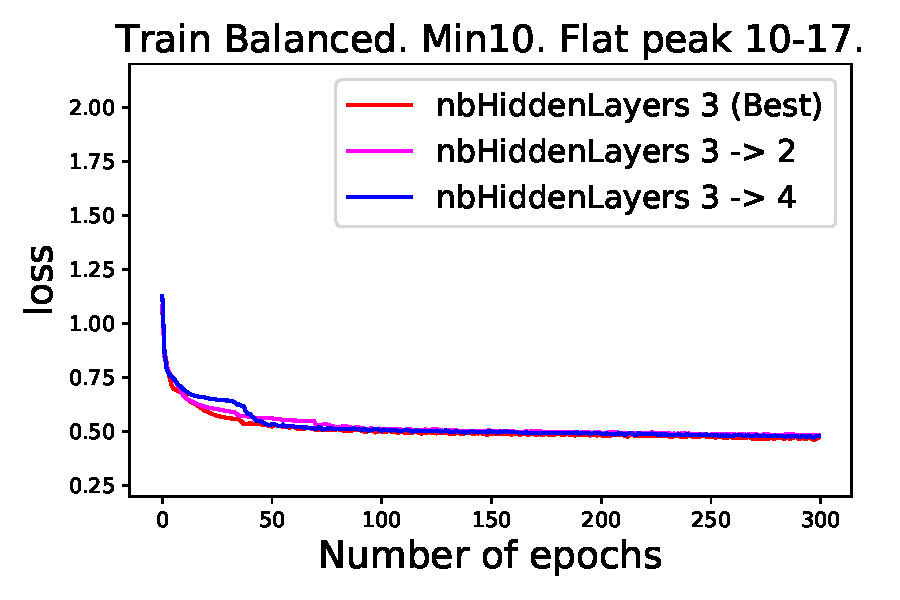
\includegraphics[width=0.32\textwidth]{plots/plot_01_1_overlay_graph_loss_Train_NbHiddenLayers.pdf}
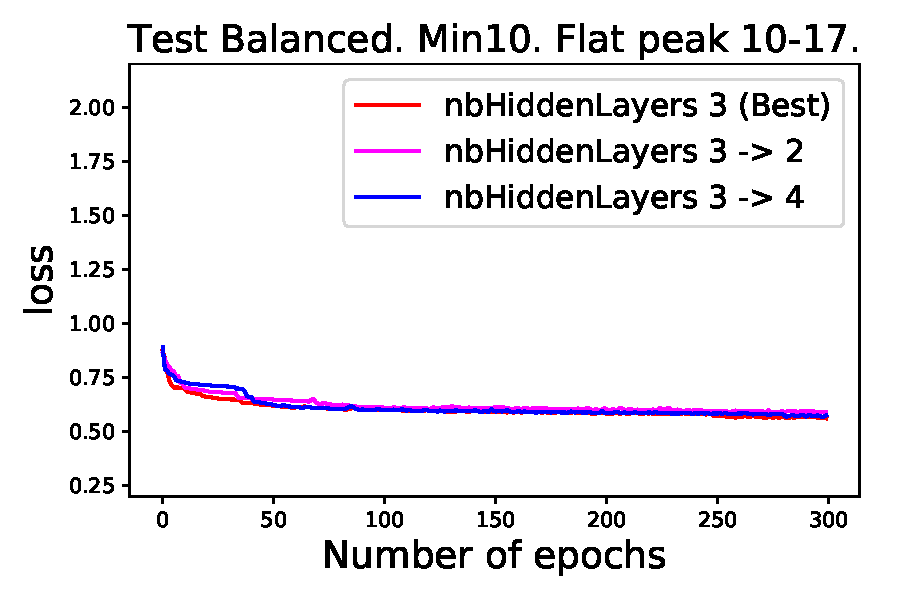
\includegraphics[width=0.32\textwidth]{plots/plot_01_1_overlay_graph_loss_Test_NbHiddenLayers.pdf}\\
\caption{Comparison of different numbers of hidden layers. 3 hidden layer is best. Binary accuracy and loss in Train and Test balanced samples.}
\label{fig:HPNbHiddenLayers}
\end{figure}

\ \\A comparison of the number of nodes on the hidden layers is studied. For simplicity, in this study it is considered the same number of nodes on each hidden layer. The performance is similar for different values, and 200 nodes on the hidden layers is retained for the final model, as illustrated in Figure~\ref{fig:HPNbNodesOnHiddenLayers}. This represents 10 times more than the nodes on the output layer.

\begin{figure}[!htb]
\centering
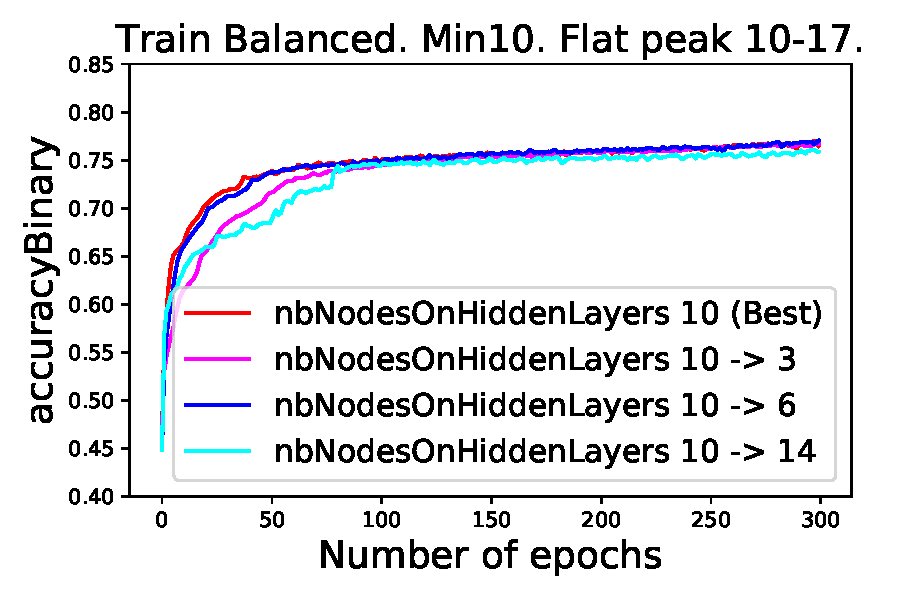
\includegraphics[width=0.32\textwidth]{plots/plot_01_1_overlay_graph_accuracyBinary_Train_NbNodesOnHiddenLayers.pdf}
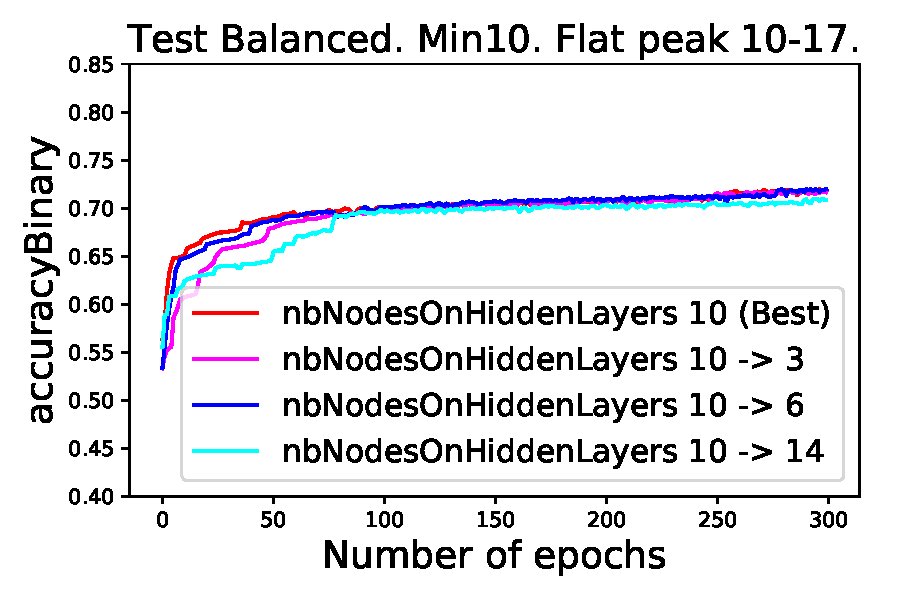
\includegraphics[width=0.32\textwidth]{plots/plot_01_1_overlay_graph_accuracyBinary_Test_NbNodesOnHiddenLayers.pdf}\\
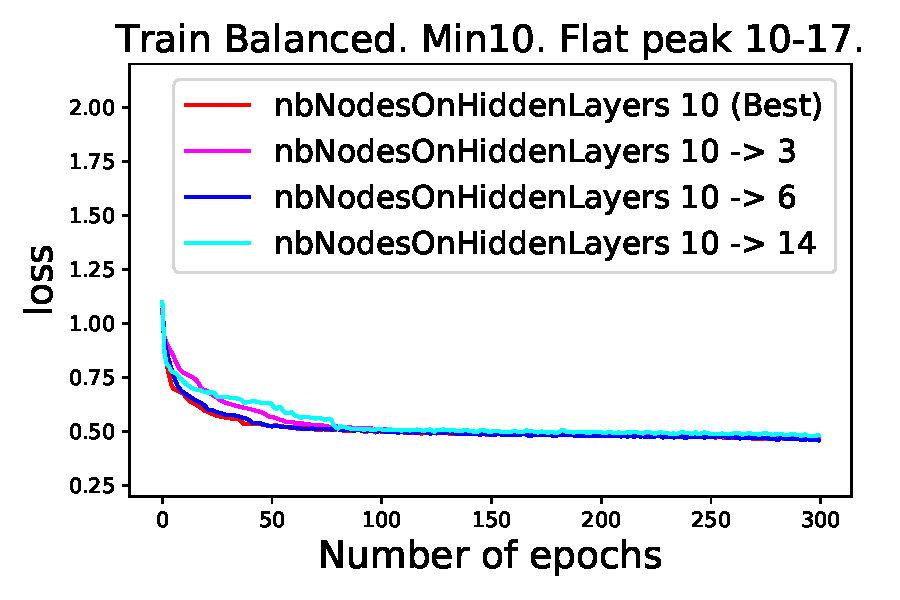
\includegraphics[width=0.32\textwidth]{plots/plot_01_1_overlay_graph_loss_Train_NbNodesOnHiddenLayers.pdf}
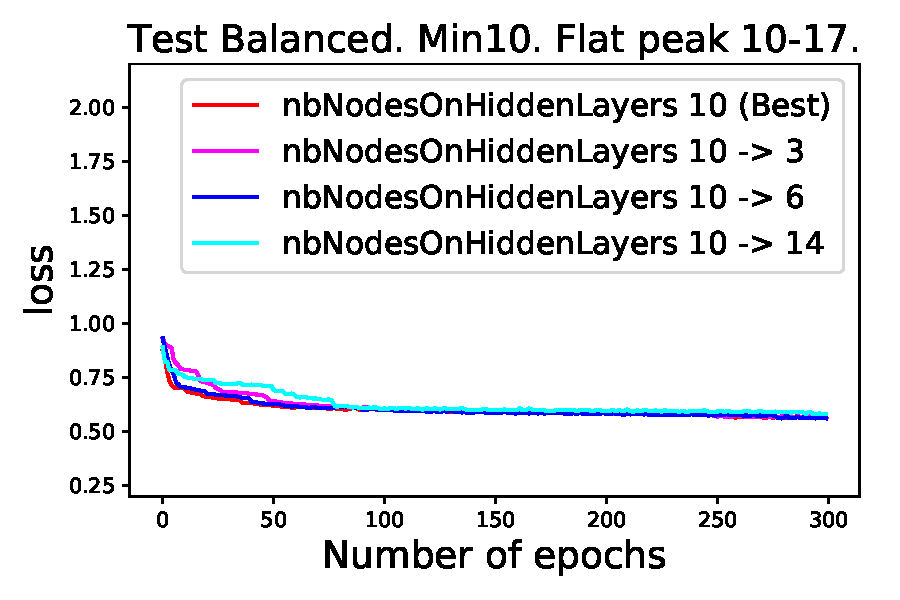
\includegraphics[width=0.32\textwidth]{plots/plot_01_1_overlay_graph_loss_Test_NbNodesOnHiddenLayers.pdf}\\
\caption{Comparison of the ratio of the different number of nodes on the hidden layers divided by the number of nodes on the last layer. k=10, or 200 nodes on each hidden layer, is best. Binary accuracy and loss in Train and Test balanced samples.}
\label{fig:HPNbNodesOnHiddenLayers}
\end{figure}

\ \\A comparison of the activation functions for the hidden layers, namely ReLU and ELU, is performed. For simplicity, in this study it is considered that all nodes of all hidden layers have the same activation function. The performance is similar between the two options, so the standard and commonly used ReLU is retained for the final model, as illustrated in Figure~\ref{fig:HPActivationFunctionHiddenLayers}.

\begin{figure}[!htb]
\centering
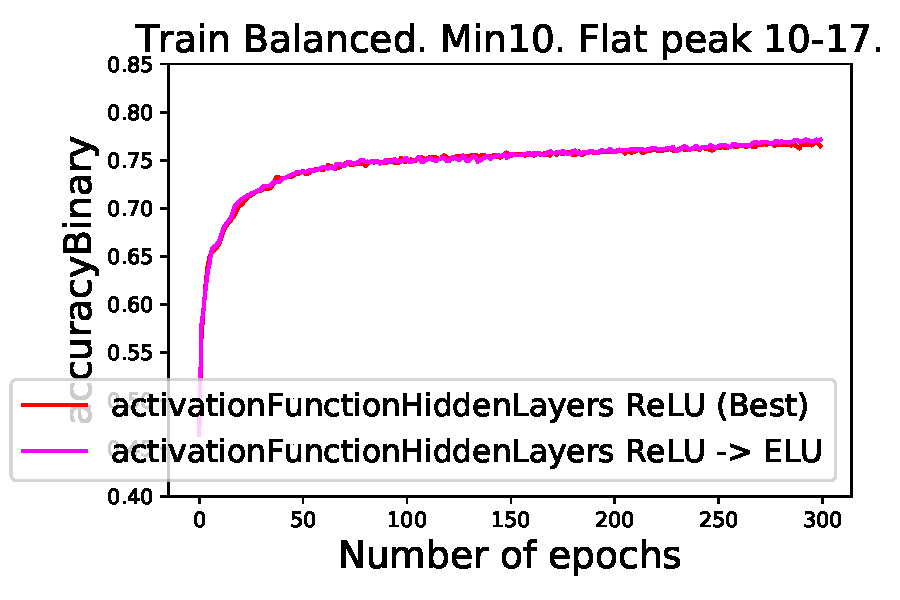
\includegraphics[width=0.32\textwidth]{plots/plot_01_1_overlay_graph_accuracyBinary_Train_ActivationFunctionHiddenLayers.pdf}
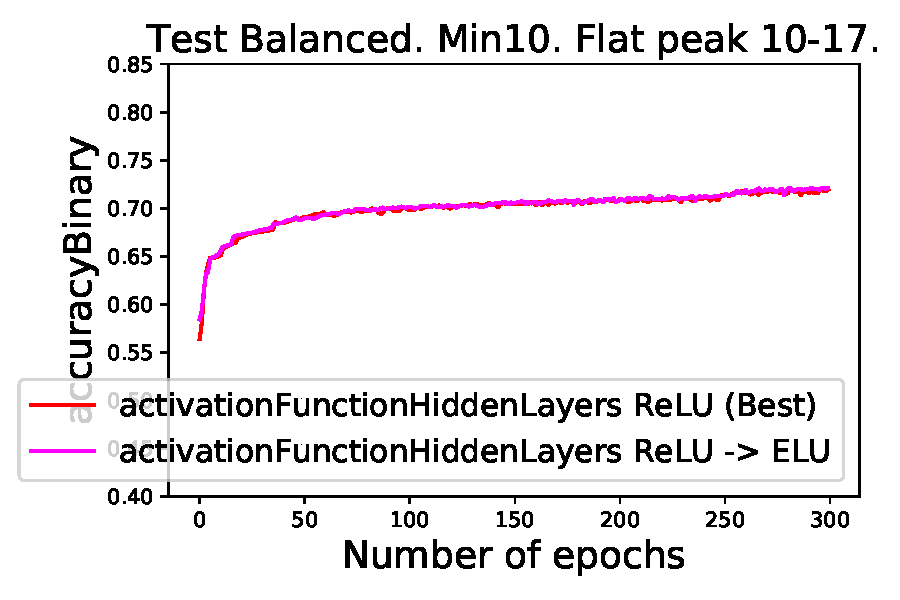
\includegraphics[width=0.32\textwidth]{plots/plot_01_1_overlay_graph_accuracyBinary_Test_ActivationFunctionHiddenLayers.pdf}\\
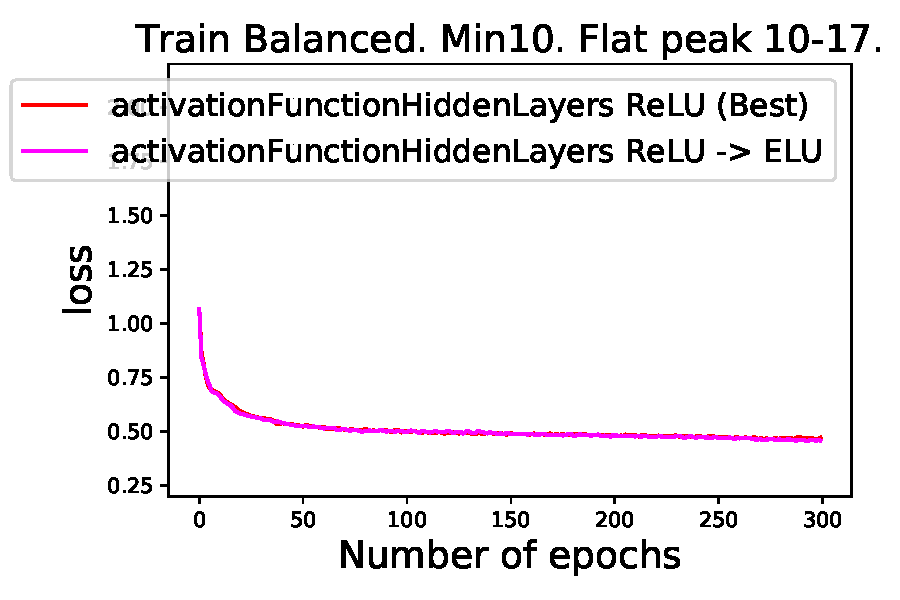
\includegraphics[width=0.32\textwidth]{plots/plot_01_1_overlay_graph_loss_Train_ActivationFunctionHiddenLayers.pdf}
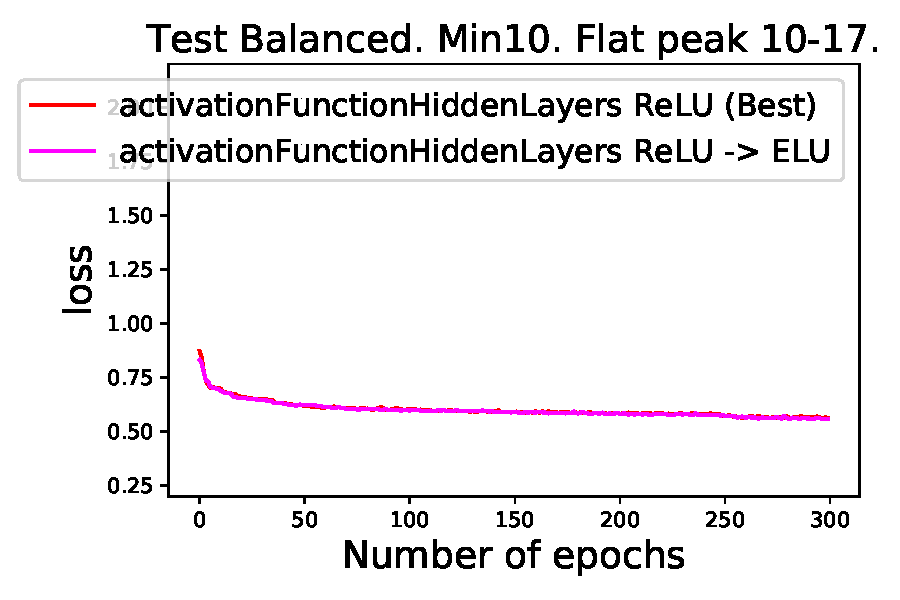
\includegraphics[width=0.32\textwidth]{plots/plot_01_1_overlay_graph_loss_Test_ActivationFunctionHiddenLayers.pdf}\\
\caption{Comparison of ReLU and ELU activation functions on the hidden layers. ReLU is chosen for the final model. Binary accuracy and loss in Train and Test balanced samples.}
\label{fig:HPActivationFunctionHiddenLayers}
\end{figure}

\ \\A comparison of adding or not adding a regularisation function via the dropout layer at the end of the hidden layers is studied. The performance is better by using a dropout layer, as illustrated in Figure~\ref{fig:HPDropoutLayer}.

\begin{figure}[!htb]
\centering
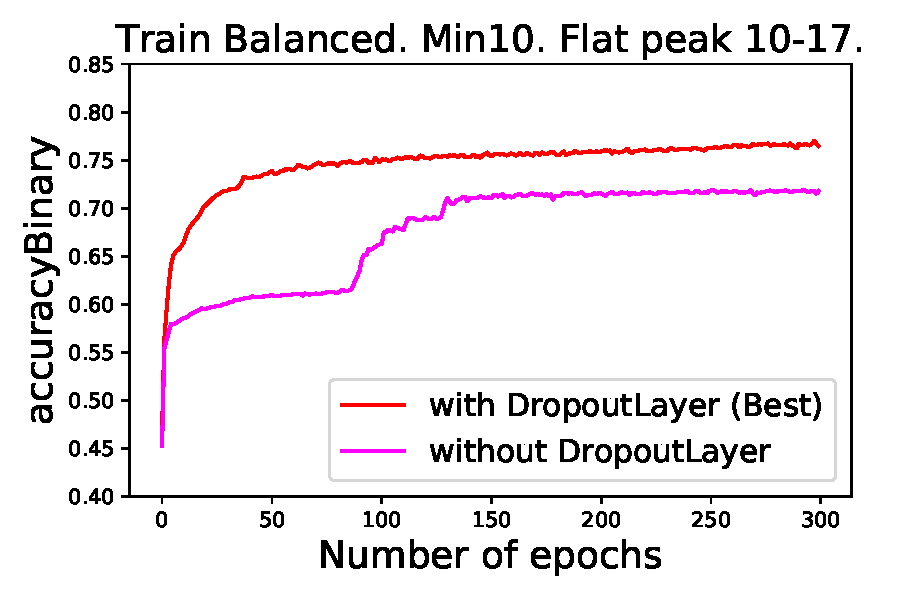
\includegraphics[width=0.32\textwidth]{plots/plot_01_1_overlay_graph_accuracyBinary_Train_DropoutLayer.pdf}
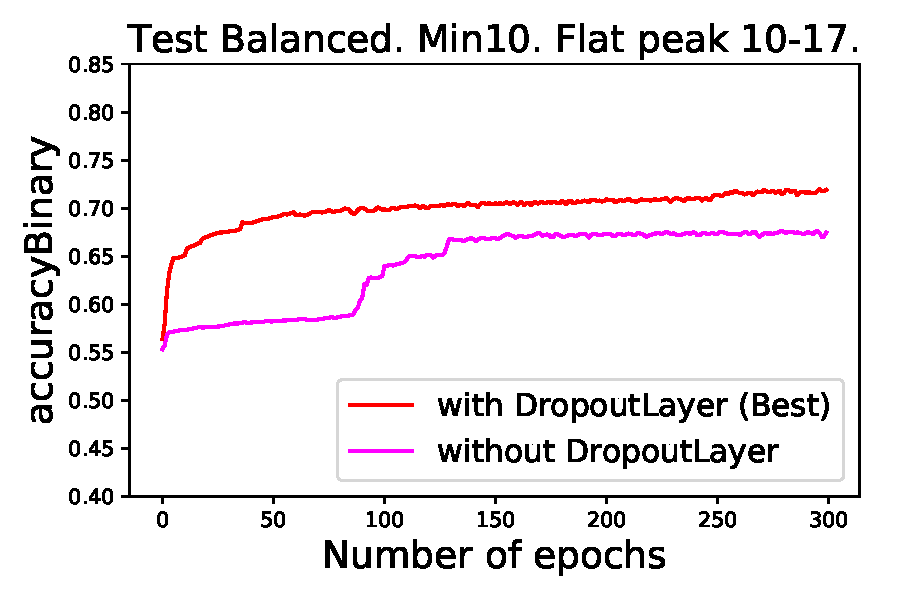
\includegraphics[width=0.32\textwidth]{plots/plot_01_1_overlay_graph_accuracyBinary_Test_DropoutLayer.pdf}\\
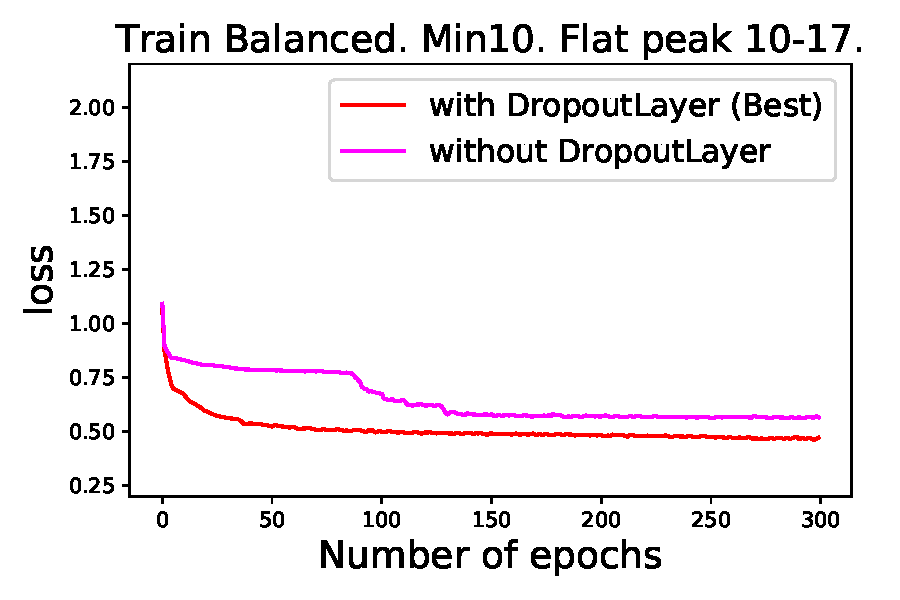
\includegraphics[width=0.32\textwidth]{plots/plot_01_1_overlay_graph_loss_Train_DropoutLayer.pdf}
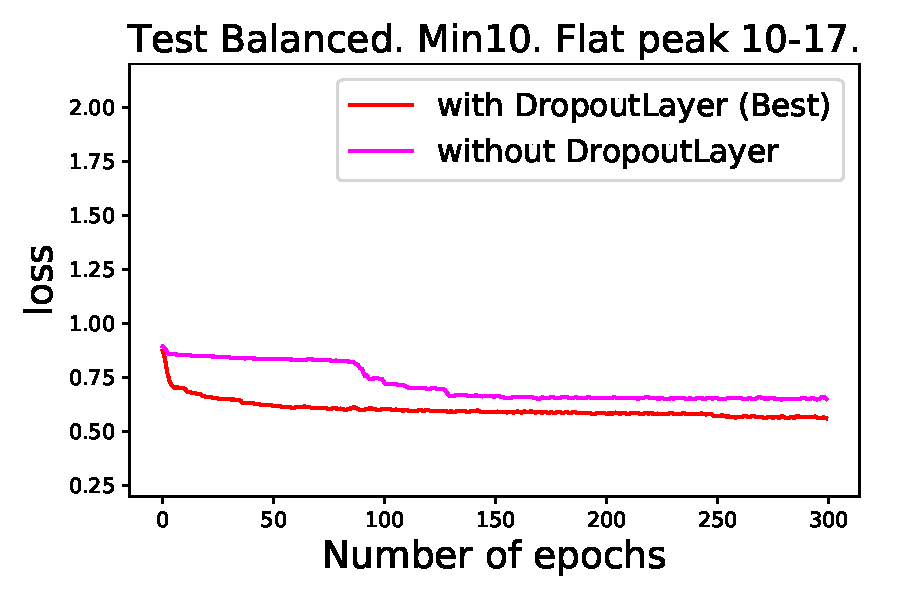
\includegraphics[width=0.32\textwidth]{plots/plot_01_1_overlay_graph_loss_Test_DropoutLayer.pdf}\\
\caption{Comparison without and with a dropout layer for regularisation. A dropout layer is used in the final model. Binary accuracy and loss in Train and Test balanced samples.}
\label{fig:HPDropoutLayer}
\end{figure}

\ \\A comparison of the activation functions for the last layer, namely TANH, SQNL and SOSI, is studied. The performance is similar for the three options, so the standard and mostly used TANH is retained for the final model, as illustrated in Figure~\ref{fig:HPActivationFunctionLastLayer}.

\begin{figure}[!htb]
\centering
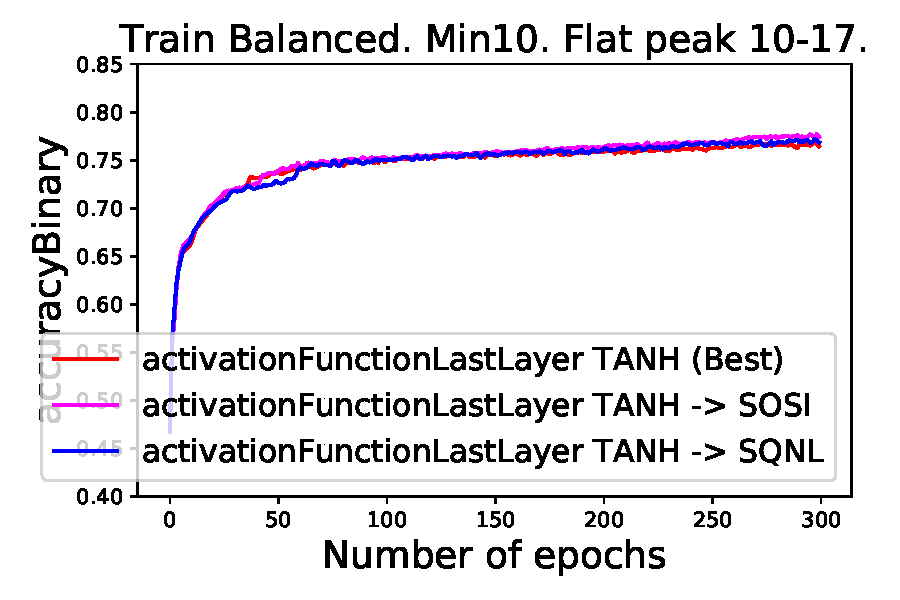
\includegraphics[width=0.32\textwidth]{plots/plot_01_1_overlay_graph_accuracyBinary_Train_ActivationFunctionLastLayer.pdf}
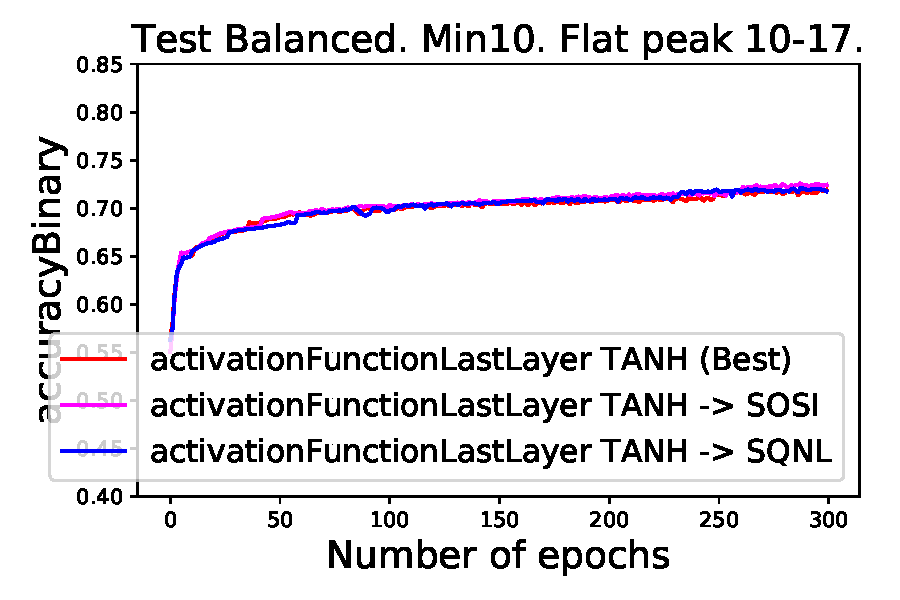
\includegraphics[width=0.32\textwidth]{plots/plot_01_1_overlay_graph_accuracyBinary_Test_ActivationFunctionLastLayer.pdf}\\
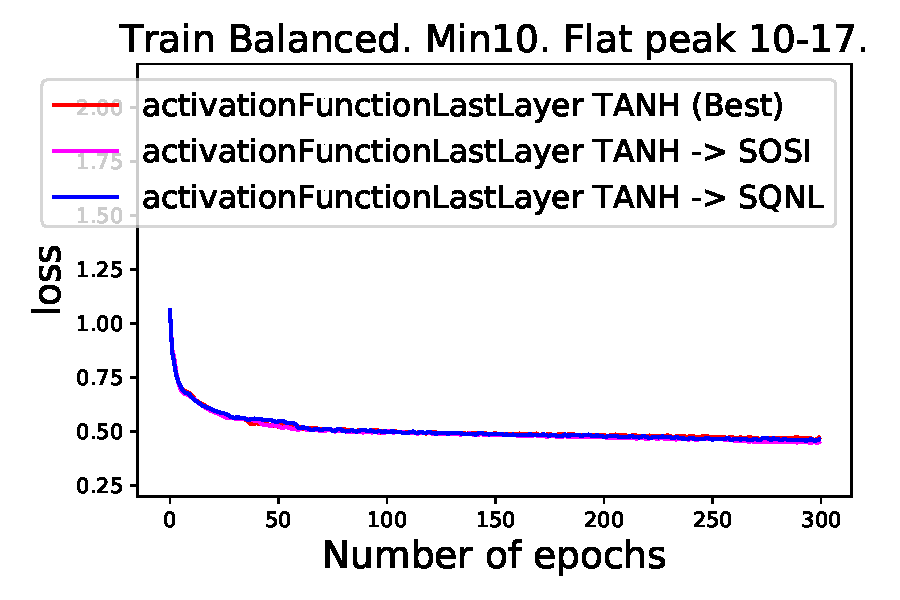
\includegraphics[width=0.32\textwidth]{plots/plot_01_1_overlay_graph_loss_Train_ActivationFunctionLastLayer.pdf}
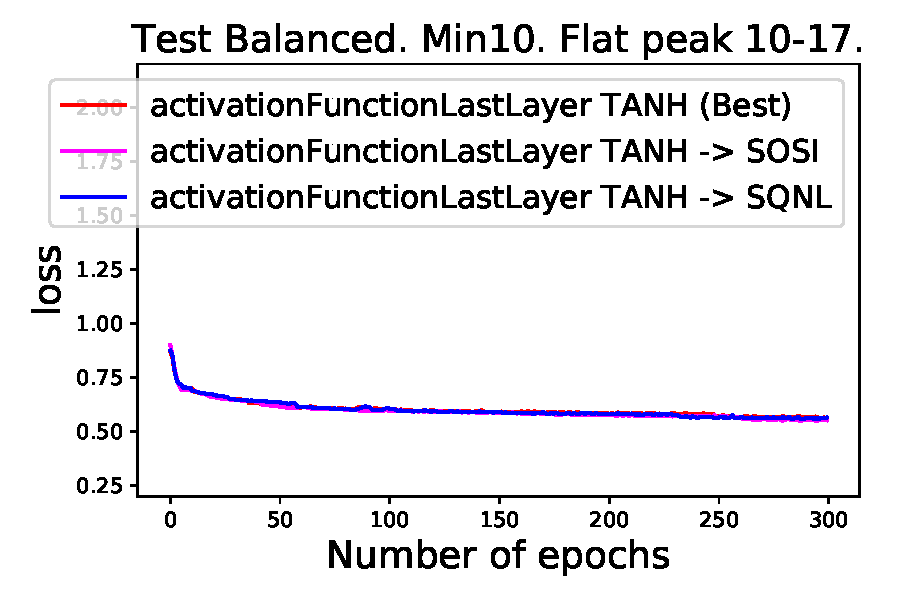
\includegraphics[width=0.32\textwidth]{plots/plot_01_1_overlay_graph_loss_Test_ActivationFunctionLastLayer.pdf}\\
\caption{Comparison of TANH, SQNL and SOSI as activation functions on the last layer. TANH is used in the final model. Binary accuracy and loss in Train and Test balanced samples.}
\label{fig:HPActivationFunctionLastLayer}
\end{figure}

\subsection{DNN Learning}
\label{sec:DNNLearning}

Moving on from the hyper-parameters that define the geometry of the deep neural network to those defining its learning method, a comparison of the optimisers, Adam and AdaDelta, each with its default parameters, is studied. The performance of Adam is significantly better than that of AdaDelta, so Adam is retained for the final model, as illustrated in Figure~\ref{fig:HPOptimizer}.

\begin{figure}[!htb]
\centering
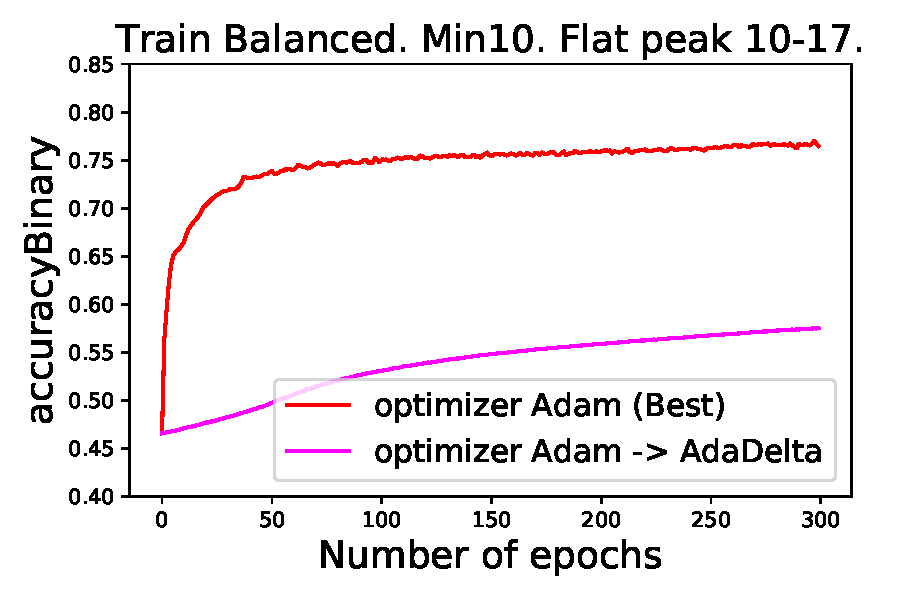
\includegraphics[width=0.32\textwidth]{plots/plot_01_1_overlay_graph_accuracyBinary_Train_Optimizer.pdf}
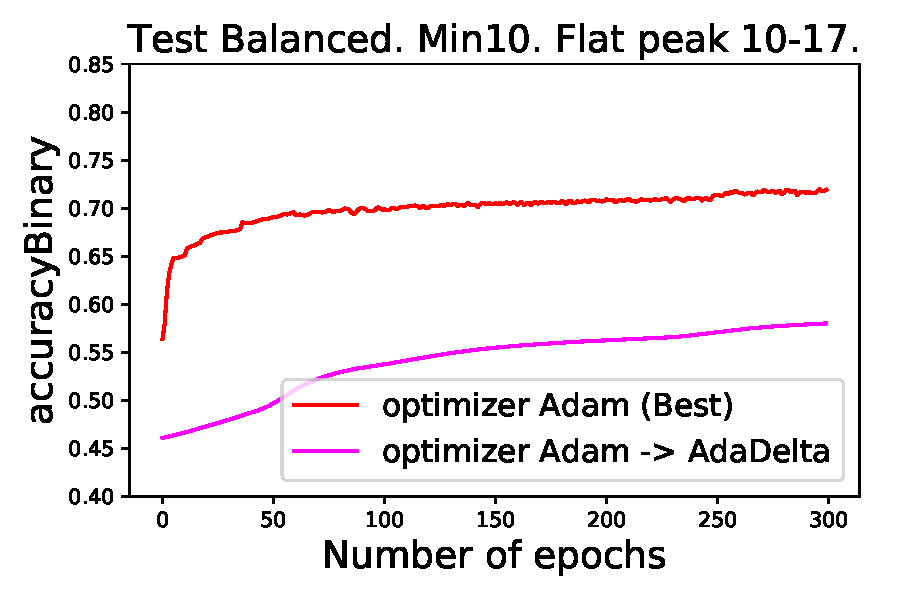
\includegraphics[width=0.32\textwidth]{plots/plot_01_1_overlay_graph_accuracyBinary_Test_Optimizer.pdf}\\
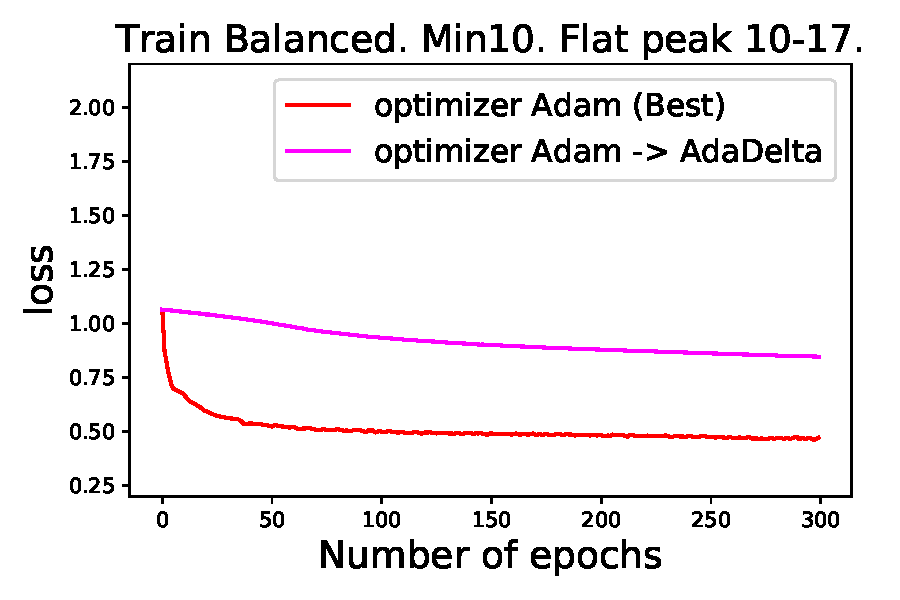
\includegraphics[width=0.32\textwidth]{plots/plot_01_1_overlay_graph_loss_Train_Optimizer.pdf}
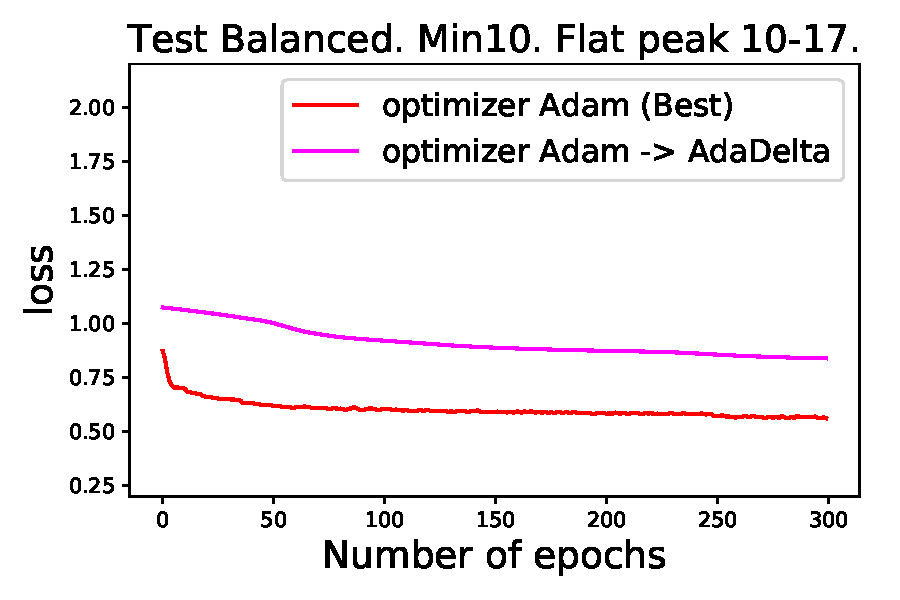
\includegraphics[width=0.32\textwidth]{plots/plot_01_1_overlay_graph_loss_Test_Optimizer.pdf}\\
\caption{Comparison of Adam and AdaDelta optimisers for the learning method. Adam is used in the final model. Binary accuracy and loss in Train and Test balanced samples.}
\label{fig:HPOptimizer}
\end{figure}

\ \\A comparison of the loss functions used to learn the weights and biases of the DNN via gradient descent, regular hinge and squared hinge, is studied. Their performance is similar, so the standard and mostly used regular hinge is retained for the final model, as illustrated in Figure~\ref{fig:HPLossFunction}.

\begin{figure}[!htb]
\centering
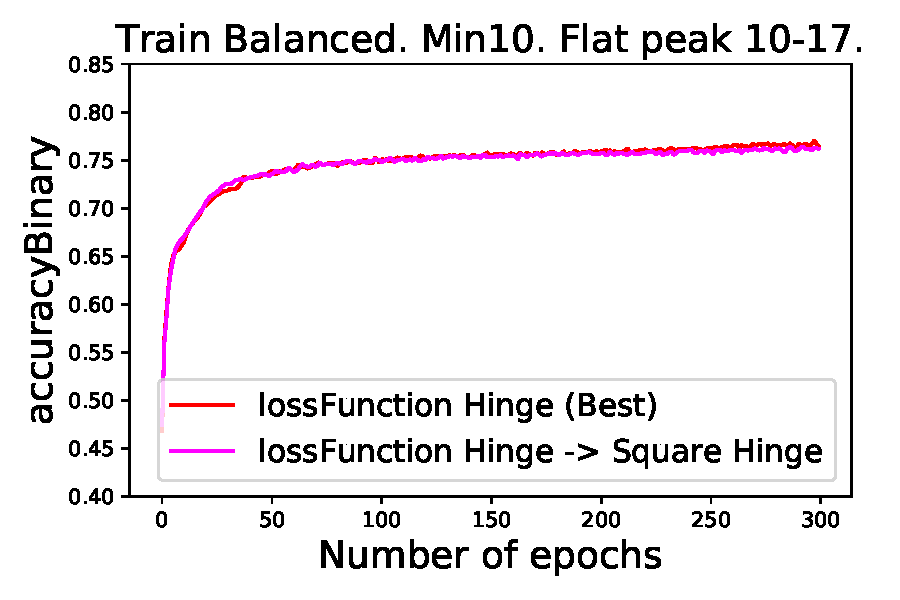
\includegraphics[width=0.32\textwidth]{plots/plot_01_1_overlay_graph_accuracyBinary_Train_LossFunction.pdf}
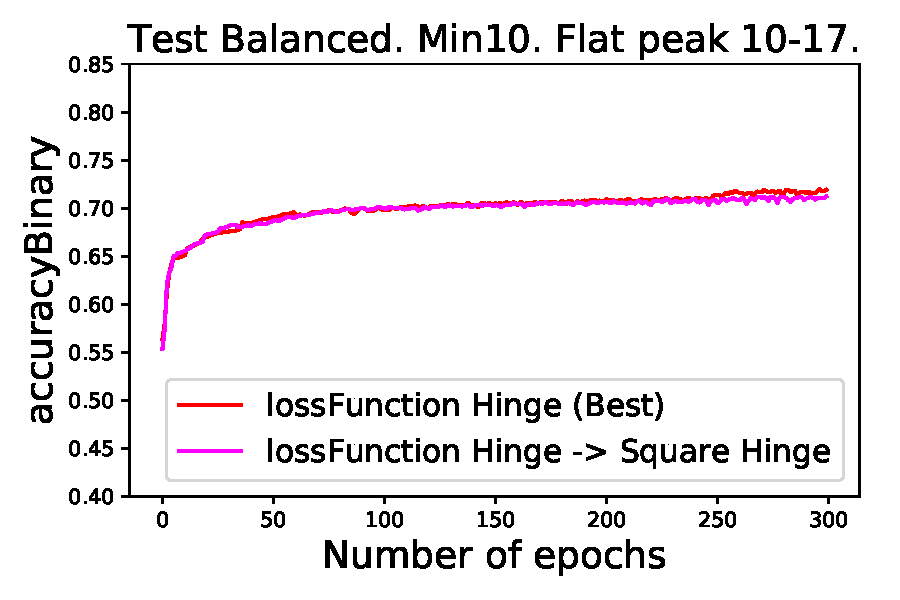
\includegraphics[width=0.32\textwidth]{plots/plot_01_1_overlay_graph_accuracyBinary_Test_LossFunction.pdf}\\
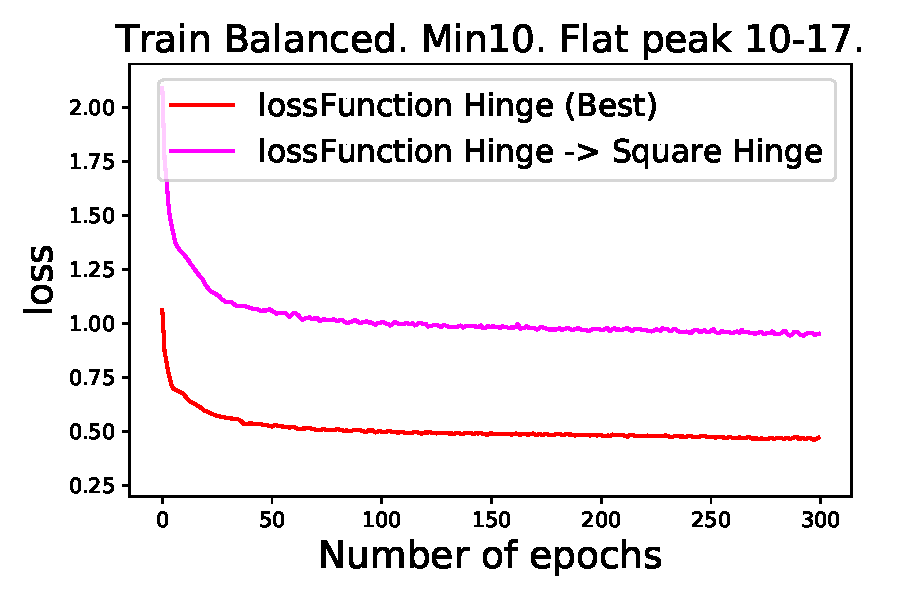
\includegraphics[width=0.32\textwidth]{plots/plot_01_1_overlay_graph_loss_Train_LossFunction.pdf}
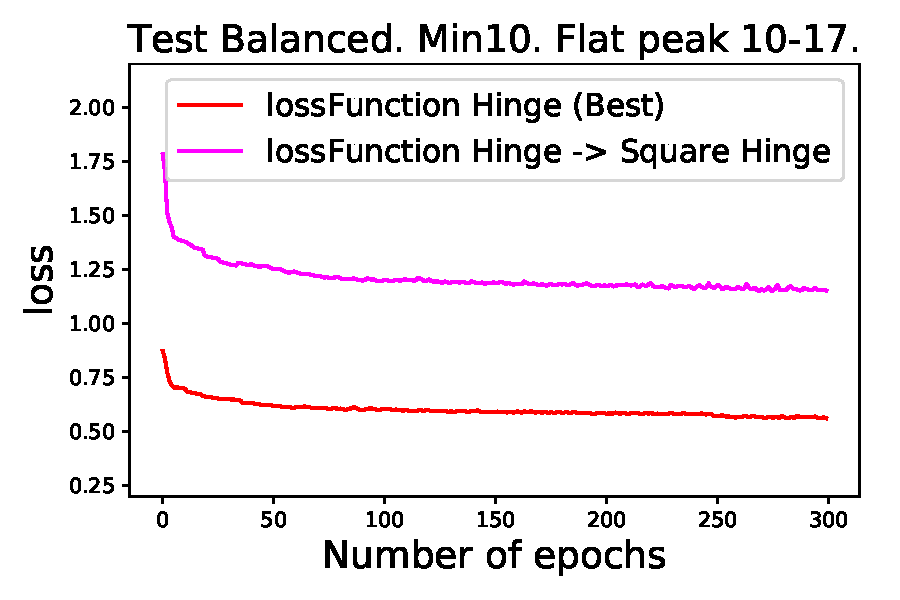
\includegraphics[width=0.32\textwidth]{plots/plot_01_1_overlay_graph_loss_Test_LossFunction.pdf}\\
\caption{Comparison of regular and square hinge loss functions for DNN learning. Regular hinge is used in the final model. Binary accuracy and loss in Train and Test balanced samples.}
\label{fig:HPLossFunction}
\end{figure}

\ \\The conclusion is that the learning part of the hyper-parameters tuning by comparing various batch sizes. The best performance is obtained for 50000, which is retained for the final model, as illustrated in Figure~\ref{fig:HPBatchSize}.

\begin{figure}[!htb]
\centering
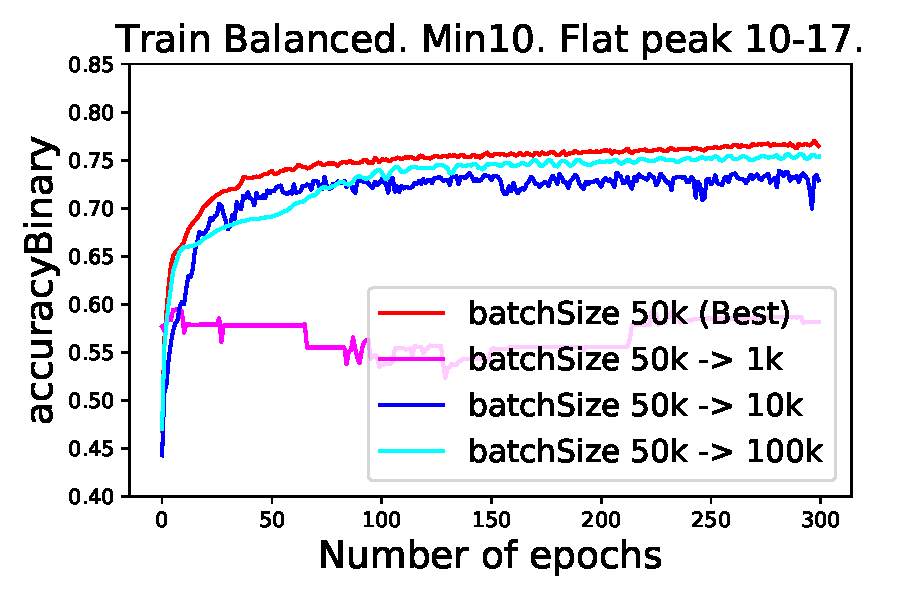
\includegraphics[width=0.32\textwidth]{plots/plot_01_1_overlay_graph_accuracyBinary_Train_BatchSize.pdf}
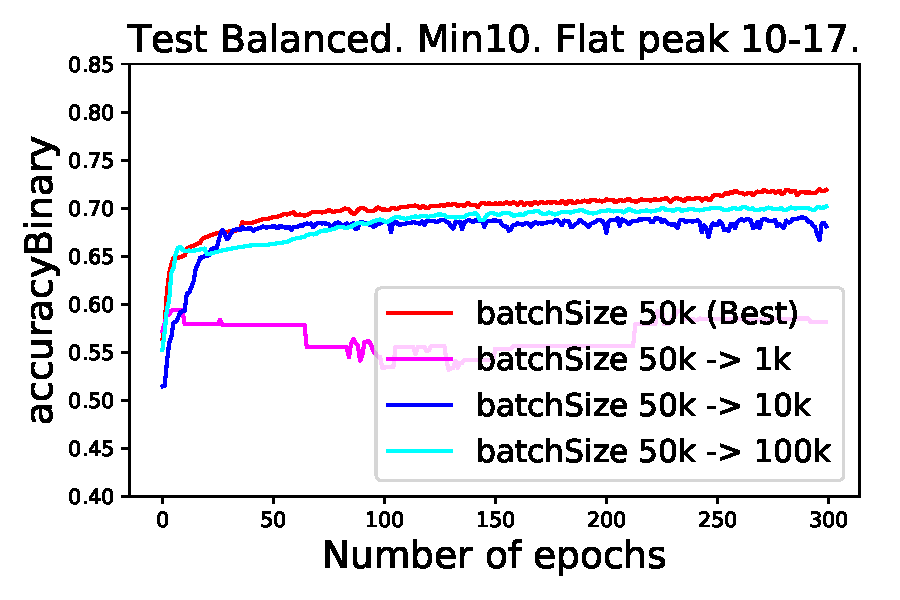
\includegraphics[width=0.32\textwidth]{plots/plot_01_1_overlay_graph_accuracyBinary_Test_BatchSize.pdf}\\
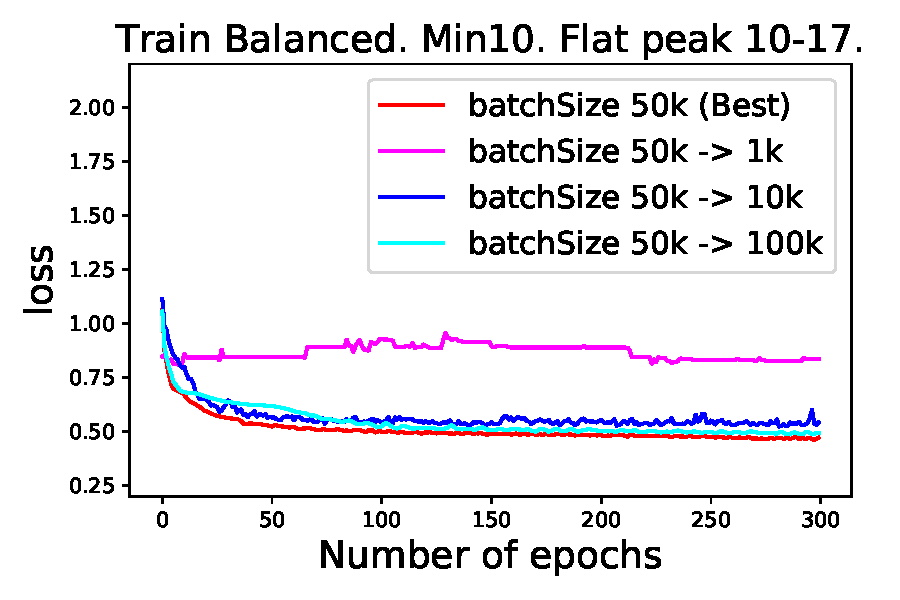
\includegraphics[width=0.32\textwidth]{plots/plot_01_1_overlay_graph_loss_Train_BatchSize.pdf}
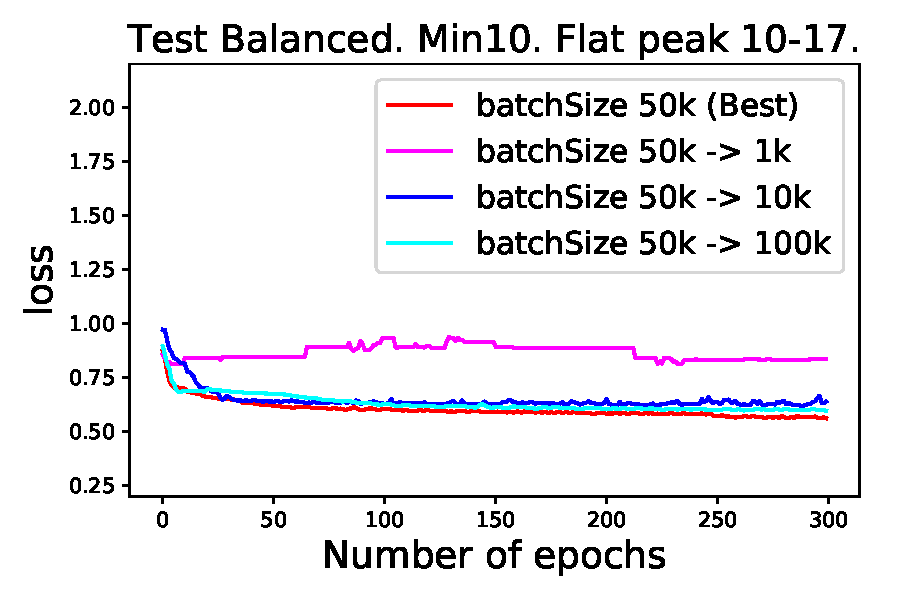
\includegraphics[width=0.32\textwidth]{plots/plot_01_1_overlay_graph_loss_Test_BatchSize.pdf}\\
\caption{Comparison of various batch sizes for DNN learning. A batch size of 50000 is used in the final model. Binary accuracy and loss in Train and Test balanced samples.}
\label{fig:HPBatchSize}
\end{figure}

\subsection{Best Model}
\label{sec:BestModel}

The problem structure fixes the number of nodes on the input layer to 60 (3 coordinates for 20 hits), and of the output layer to 20 (1 boolean for 20 hits). The DNN architecture and learning methods are optimised as hyper-parameters, whose options are limited by the choice of representing the answers yes and no by 1.0 and -1.0, respectively. The hyper-parameters that describe the best model are summarised as follows.

\ \\There are 3 hidden layers, each with 200 nodes, or 10 times more than the number of nodes in the output layer. A reminder is that the input layer has 60 nodes (3 coordinates x, y, z for each of the 20 hits in the bucket) and the output layer has 20 nodes (an output of -1.0 or 1.0 for each of the 20 hits in the bucket). A dropout layer (0.2) is added at the end of the hidden layers. The activation function for the hidden layers is the rectified linear unit (ReLU). The activation function for the last layer is hyperbolic tangent ($\tanh$). The loss function is the (regular) hinge function. The batch size is 50000.

\ \\While the choice of hyper-parameters is done using 300 epochs and the balanced test dataset, the final result uses 1200 epochs and the unbalanced test dataset.

\section{Predicting or Inference and Figures of Merit}

Once the model is trained, it can be applied to a new dataset to infer or make a prediction.

\ \\Besides the value of the loss function across the entire dataset, there is also another figure of merit of how well does a NN perform in training and testing. It is called \emph{accuracy} and is related to the number of of true positives or false negatives. The larger the accuracy, the better.

\ \\For the training dataset, the loss and accuracy values always improve. But in the testing dataset they can start to degrade if we train for too many epochs. By degrading it means that the loss value starts to grow, and the accuracy value starts to decrease. That is called over-training and consists of memorizing the inputs, and thus not being able to predict correctly any more for new inputs.

\ \\The confusion matrix is a table that summarises the performance of a binary classification model, as illustrated in Table~\ref{tab:ConfusionMatrix}. 

\begin{table}[h!]
 \centering
   
    \begin{tabular}{|l|l|} % <-- Alignments: 1st column left, 2nd middle and 3rd right, with vertical lines in between
      \hline
      TP & FP \\
      \hline
      FN & TN \\
      \hline
    \end{tabular}
\caption {Confusion Matrix.}
\label{tab:ConfusionMatrix}
\end{table}

\ \\The four metrics presented in the table are true positive (TP), false positive (FP), false negative (FN), and true negative (TN). Based on these four numbers further figures of merit are derived.

\ \\The accuracy defines what percentage of the total predictions are classified correctly, either as TP or TN, as defined by the Equation

\begin{equation}
   \Accuracy = \frac{\TP + \TN}{\TP + \TN + \FP + \FN}.
\end{equation}

\ \\The precision defines the percentage of the predicted positive that are actually positive, as defined by Equation

\begin{equation}
   \Precision = \frac{\TP}{\TP + \FP}.
\end{equation}

\ \\The recall defines the percentage of actual positive that are correctly predicted, as defined by the Equation

\begin{equation}
   \Recall = \frac{\TP}{\TP + \FN}.
\end{equation}

\ \\ The equivalents of the precision and recall can be constructed also for the negative values, as if the negative values are the sought target. The negative predicted value is the negative equivalent of precision and it represents the percentage of the predicted negative that in reality are also negative, as defined by Equation

\begin{equation}
   \NegativePredictedValue = \frac{\TN}{\TN + \FN}.
\end{equation}

\ \\The true negative rate is the negative equivalent of the recall. It defines the percentage of the real negative that are also predicted as negative, as defined by Equation 

\begin{equation}
   \TrueNegativeRate = \frac{\TN}{\TN + \FP}.
\end{equation} 

\ \\The pseudo-code to calculate the metrics is described in Appendix~\ref{sec:AppendixModelEvaluationMetrics}. 

\section{Software Used}

Several software Python libraries are used to perform this study, including data manipulation, the NN training, the figure of merit evaluation and plotting.

\ \\Numpy is a Python programming library, which is a coding support for large multi-dimensional arrays and matrices~\cite{Numpy}. 

\ \\PANDAS is a data manipulation and analysis library~\cite{PANDAS}. It is an open source library that is made mainly for working with relational or labeled data. It provides various data structures and operations for manipulating numerical data and time series. It is fast, has high performance and productivity. A data frame is a two-dimensional data structure with labeled data (rows and columns). Pandas uses numpy behind the hood. 

\ \\Jupyter Notebook is an important tool in the data science field. It is a web-based interactive computing platform~\cite{JupyterNotebook}. The Notebook combines code, equations, text, visualisation, interactive dashboard and other media. It works in line code, using blocks. 

\ \\Matplotlib is used for producing the plots in this thesis, both 1D and 2D~\cite{Matplotlib}.


